\documentclass[14pt]{article}

\usepackage[letterpaper,bindingoffset=0.2in,%
            left=1in,right=1in,top=1in,bottom=1in,%
            footskip=.25in]{geometry}
\usepackage[english]{babel}
\usepackage[utf8x]{inputenc}
\usepackage{amsmath}
\usepackage{amssymb}
\usepackage{amsthm}
\usepackage{graphicx}
\usepackage[makeroom]{cancel}
\usepackage{booktabs}
\usepackage{enumitem}
\usepackage{tabularx}
\usepackage{xcolor}
\usepackage{hyperref}
\usepackage{tikz}
\usepackage{pgfplots}
\pgfplotsset{compat=1.11}
\usepackage{systeme}
\usepackage{calc}
\usepackage{caption}
\usepackage{subcaption}
\usepackage{multicol}
\usepackage{listings}

\lstset{language=Python}

\usetikzlibrary{calc}
\usetikzlibrary{positioning}
\usetikzlibrary{arrows,decorations.markings}

\graphicspath{ {./images/} }


% DOCUMENT STARTS HERE

\begin{document}

\title{Analysis H Project: \\ \textbf{3D Graphics Generation with Matrices}}
\author{Mihir Rao}
\maketitle

\begin{center}
	\vspace{3em}
	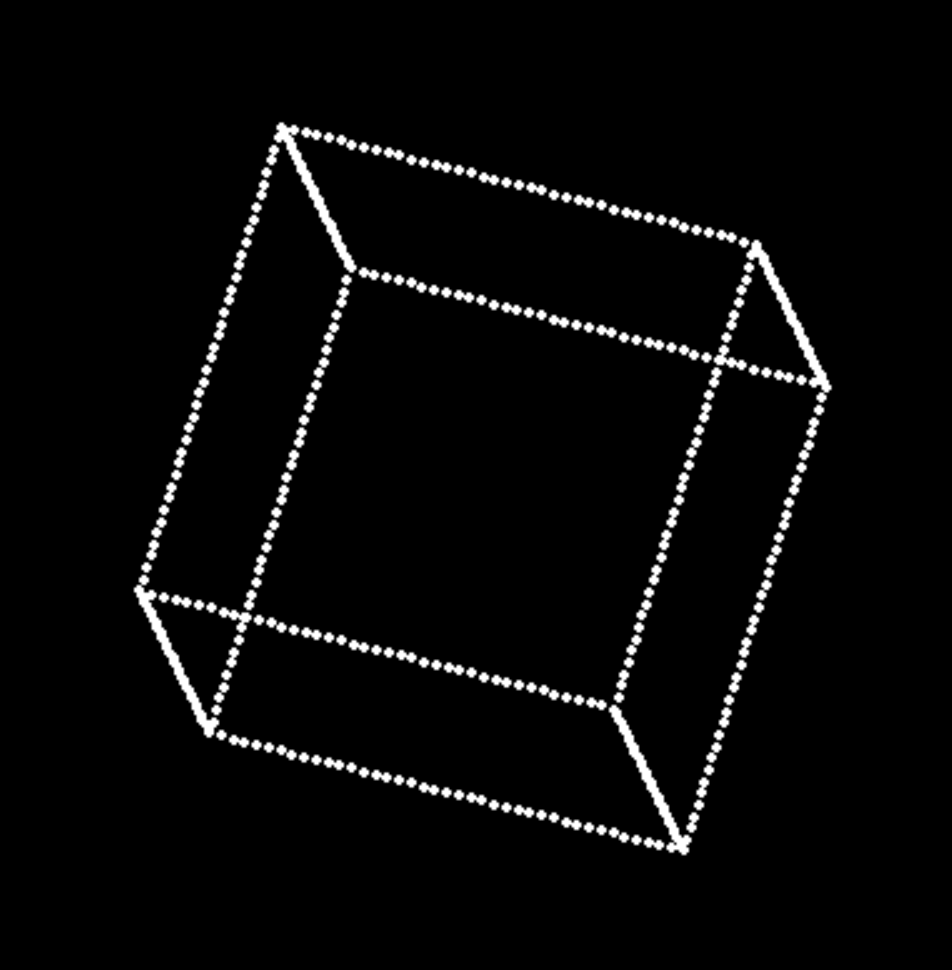
\includegraphics[scale=0.8]{titleImg}
	\vspace{3em}
\end{center}

\section*{Overview}

For our Analysis H project, Steve and I decided to dive into the realm of computer graphics and matrices' applications in this field. Specifically, we wrote code that generates 3D points, projects these 3D points onto a 2D surface(the computer screen), and transforms these points to display an animation(using matrices). We both were fascinated by the numerous applications of matrices and thought this will be a fun project to work on. After doing further research, it also turns out that Renderman, Pixar's animation software, is heavily based on matrices and linear algebra; so this was the perfect time for us to dip our toes in the fundamentals of this field. This document serves to explain how we came up with the math of this code, challenges we faced, and the ultimate solutions to those challenges. The next section is a brief introduction of how we approached the code and following that is the actual math behind it. Enjoy!

\newpage

\section*{Introduction}

For this project, we developed 3 main functions in the code that do the majority of the heavy lifting in terms of displaying the object on the screen. The first one is the generatePoints function, followed by the pointsBetween function, and lastly the big one: createCompositeMatrix.

\section*{The Math}

Math stuff.

\end{document}